%!TEX root = ../../main.tex

% supp3

\section{Baird's advantage-learning investigation}
\label{bairdal}

\begin{figure}[H]
  \center\scalebox{0.12}[0.12]{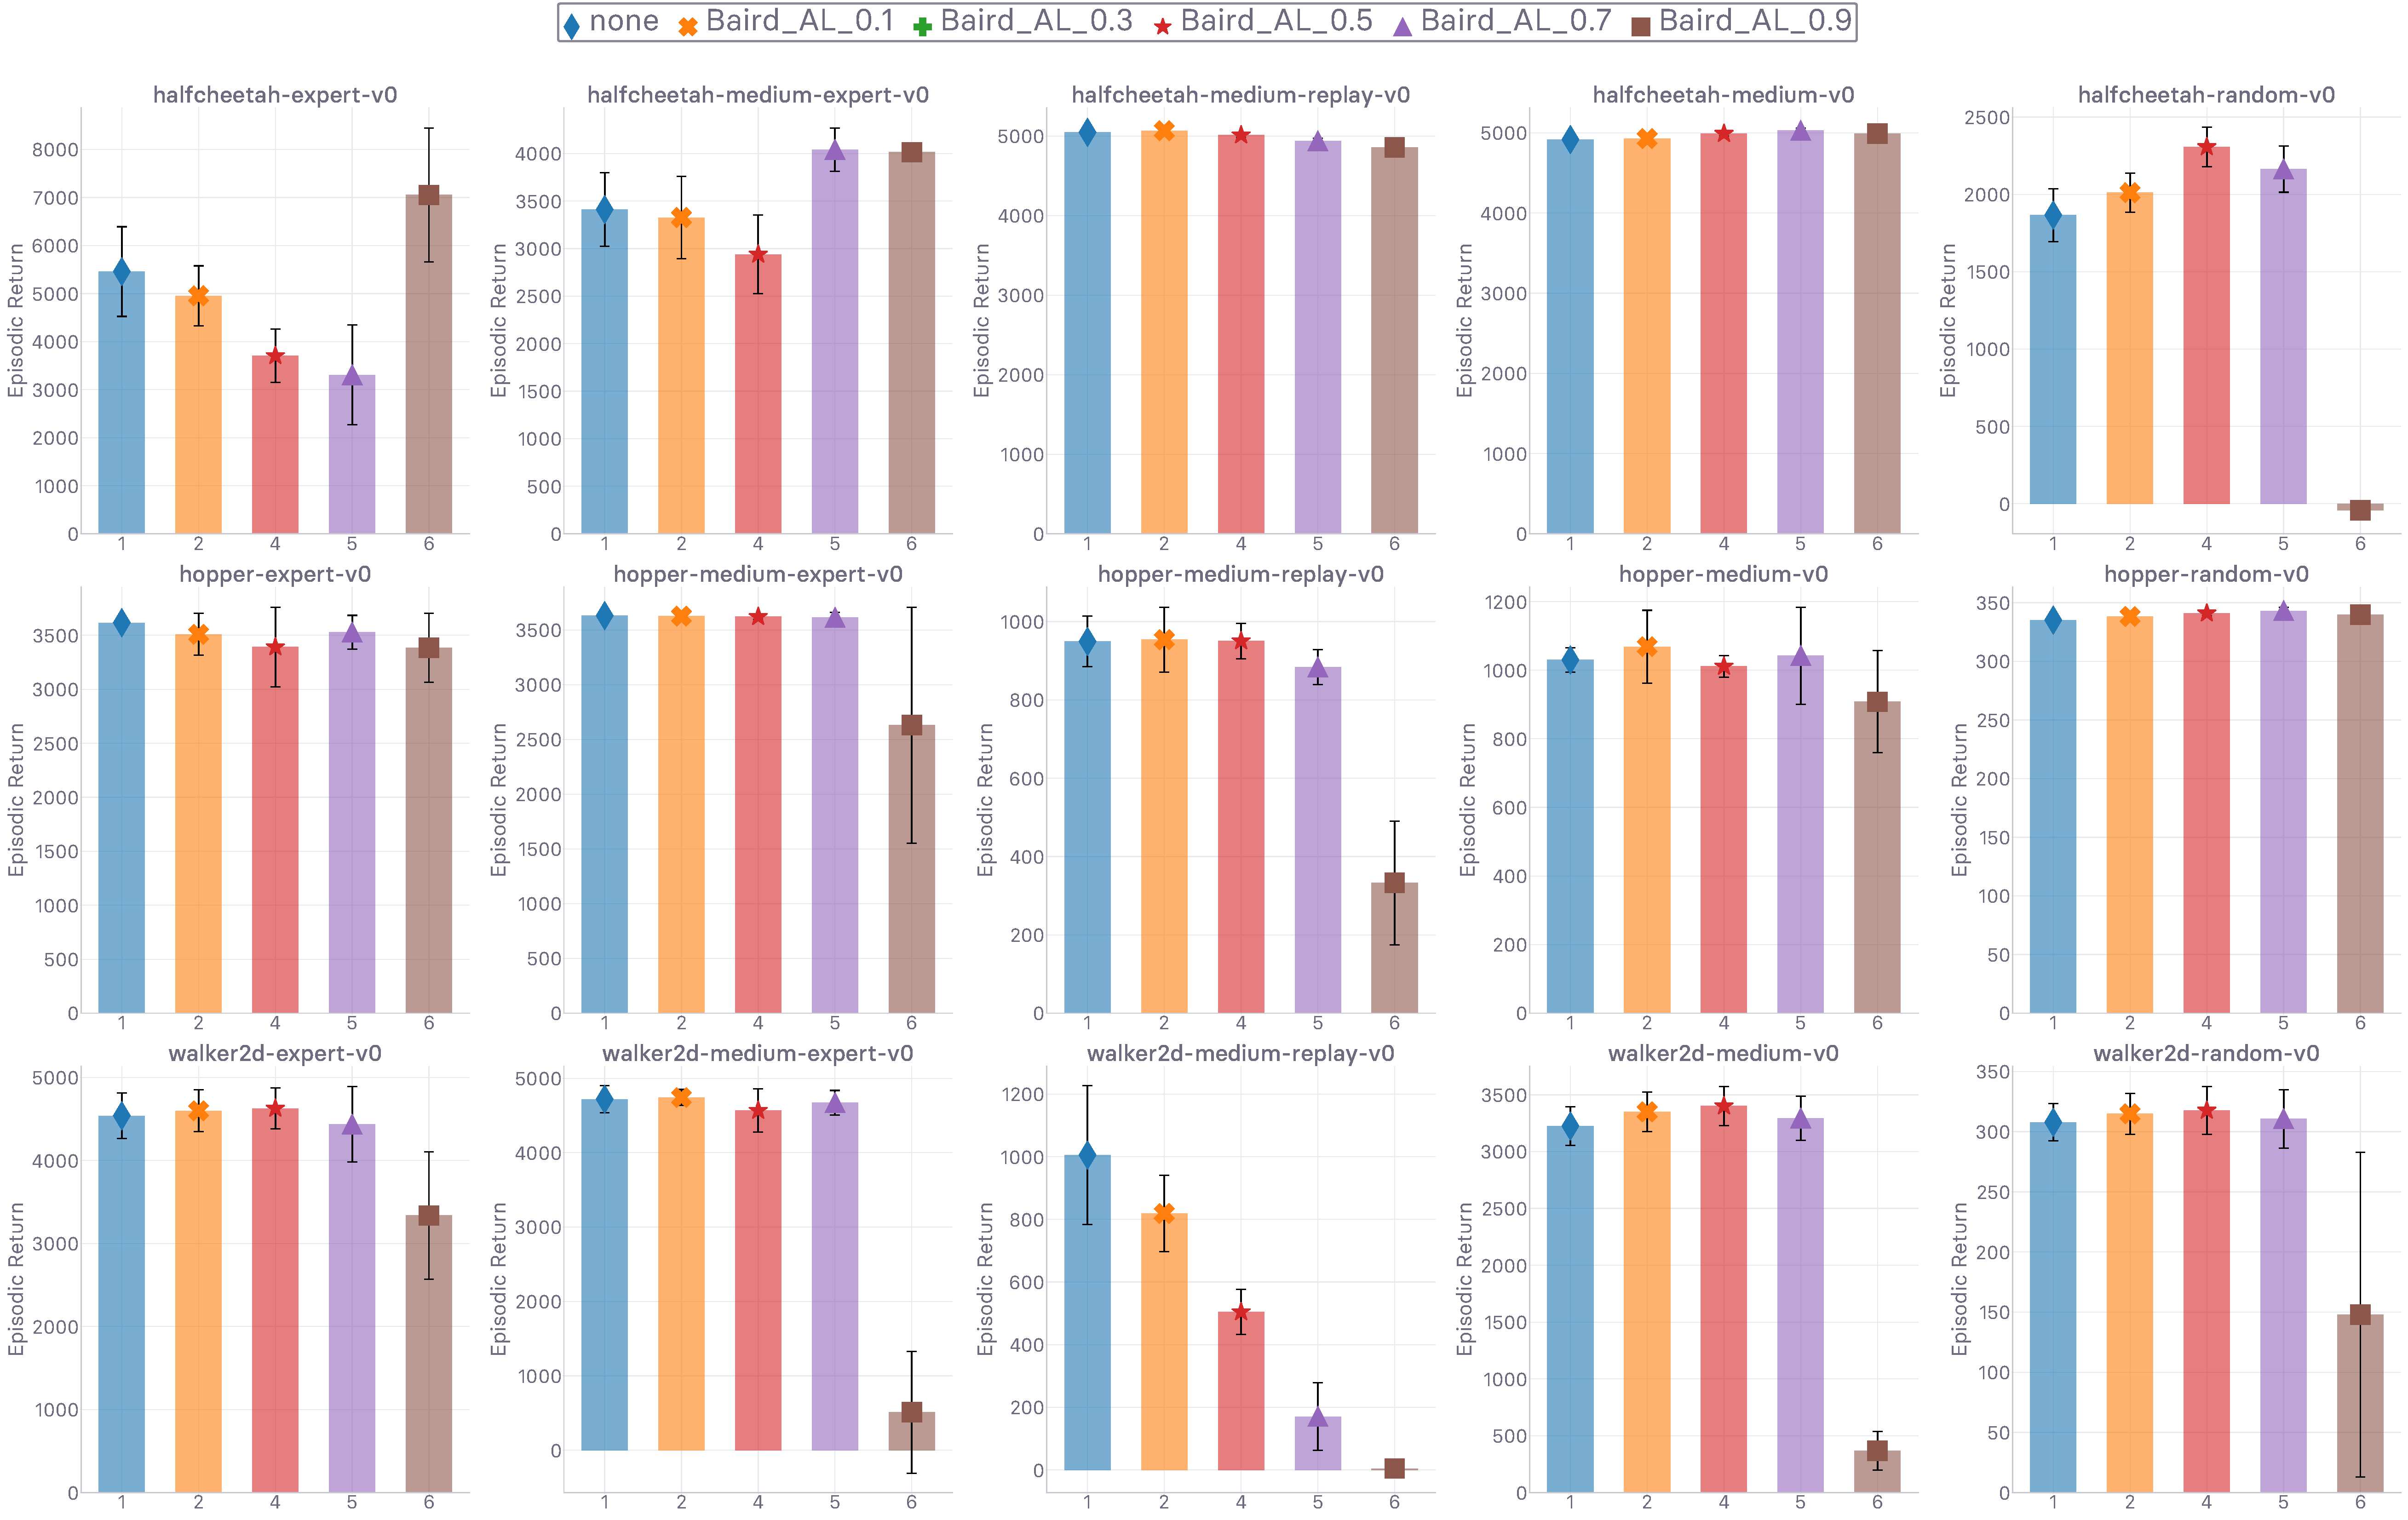
\includegraphics{Plots/baird_al/plots_main_eval_env_ret_barplot.pdf}}
  \caption{Empirical evaluation of the use of Baird's advantage-learning bonus (\textit{cf.}~\ref{criticlossal}),
  and sweep over the associated scaling coefficient $\alpha$.
  Runtime is 12 hours. Best seen in color.}
  \label{bairdal:barplot}
\end{figure}

\section{Proposal involving $\mathcal{T}_\textsc{Max}^{\omega, m}$ in policy evaluation}
\label{tmaxops}

\begin{figure}[H]
  \center\scalebox{0.12}[0.12]{\includegraphics{Plots/next_max_m_sweep/%
  beta_clone_max/plots_main_eval_env_ret_barplot.pdf}}
  \caption{Sweep over the number of samples $m$ used in the operator
  $\mathcal{T}_\textsc{Max}^{\omega', m}\big[\beta_\textsc{c}\big]$
  (\textit{cf.}~\textsc{Section}~\ref{operators}, \ref{betaclonemax}).
  Runtime is 12 hours. Best seen in color.}
  \label{betaclonemaxm:barplot}
\end{figure}
\begin{figure}[H]
  \center\scalebox{0.12}[0.12]{\includegraphics{Plots/next_max_m_sweep/%
  perturbed_beta_clone_max/plots_main_eval_env_ret_barplot.pdf}}
  \caption{Sweep over the number of samples $m$ used in the operator
  $\mathcal{T}_\textsc{Max}^{\omega', m}\big[\beta_\textsc{c}^\xi\big]$
  (\textit{cf.}~\textsc{Section}~\ref{operators}, \ref{perturbedbetaclonemax}).
  Runtime is 12 hours. Best seen in color.}
  \label{perturbedbetaclonemaxm:barplot}
\end{figure}
\begin{figure}[H]
  \center\scalebox{0.12}[0.12]{\includegraphics{Plots/next_max_m_sweep/%
  theta_max/plots_main_eval_env_ret_barplot.pdf}}
  \caption{Sweep over the number of samples $m$ used in the operator
  $\mathcal{T}_\textsc{Max}^{\omega', m}[\pi_\theta]$
  (\textit{cf.}~\textsc{Section}~\ref{operators}, \ref{thetamax}).
  Runtime is 12 hours. Best seen in color.}
  \label{thetamaxm:barplot}
\end{figure}

\section{Policy improvement objective derivation}
\label{agentobjectivedetail}

We begin with the \emph{forward} KL, by unpacking the measure and the expectations into explicit integral form,
and injecting \textsc{eq}~\ref{pistar}:
\begin{align}
  \mathbb{E}_{s \sim \rho^\beta(\cdot)}
  \Big[
  \Delta\big(\pi_\theta(\cdot | s), \zeta_\textsc{iw}(\cdot | s)\big)
  \Big]
  &\coloneqq
  \mathbb{E}_{s \sim \rho^\beta(\cdot)}
  \Big[
  D^{\zeta_\textsc{iw}}_{\overrightarrow{\textsc{kl}}}[\pi_\theta](s)
  \Big]
  \\
  &= \int_{s \in \mathcal{S}} \rho^\beta(s) \int_{a \in \mathcal{A}} \zeta_\textsc{iw}(a | s)
  \big(\log \zeta_\textsc{iw}(a | s) - \log \pi_\theta(a | s)\big) \, da \, ds
  \\
  &= \int_{s \in \mathcal{S}} \rho^\beta(s) \int_{a \in \mathcal{A}} \zeta_\textsc{iw}(a | s)
  \log \zeta_\textsc{iw}(a | s) \, da \, ds \nonumber \\
  & \qquad -
  \int_{s \in \mathcal{S}} \rho^\beta(s) \int_{a \in \mathcal{A}} \zeta_\textsc{iw}(a | s)
  \log \pi_\theta(a | s) \, da \, ds
\end{align}
\begin{align}
  \implies \quad
  \theta &\coloneqq
  \argmin_{\theta \in \Theta} \;\,
  \mathbb{E}_{s \sim \rho^\beta(\cdot)}
  \Big[
  \Delta\big(\pi_\theta(\cdot | s), \zeta_\textsc{iw}(\cdot | s)\big)
  \Big]
  \\
  &= \argmin_{\theta \in \Theta} \;\,
  - \int_{s \in \mathcal{S}} \rho^\beta(s) \int_{a \in \mathcal{A}}
  \zeta_\textsc{iw}(a | s)
  \log \pi_\theta(a | s) \, da \, ds \\
  &= \argmin_{\theta \in \Theta} \;\,
  - \int_{s \in \mathcal{S}} \rho^\beta(s) \int_{a \in \mathcal{A}}
  \zeta(a | s) \exp (\frac{1}{\lambda_\textsc{kl}} A^{\pi_\theta}_\omega(s,a))
  \log \pi_\theta(a | s) \, da \, ds \\
  &= \argmax_{\theta \in \Theta} \;\,
  \mathbb{E}_{s \sim \rho^\beta(\cdot), a \sim \zeta(\cdot | s)}
  \bigg[
  \exp (\frac{1}{\lambda_\textsc{kl}} A^{\pi_\theta}_\omega(s,a)) \log \pi_\theta(a | s)
  \bigg]
\end{align}
Conversely, by opting for the \emph{reverse} KL instead, the problem in \textsc{eq}~\ref{pistar}
reduces to the following problem:
\begin{align}
  \mathbb{E}_{s \sim \rho^\beta(\cdot)}
  \Big[
  \Delta\big(\pi_\theta(\cdot | s), \zeta_\textsc{iw}(\cdot | s)\big)
  \Big]
  &\coloneqq
  \mathbb{E}_{s \sim \rho^\beta(\cdot)}
  \Big[
  D^{\zeta_\textsc{iw}}_{\overleftarrow{\textsc{kl}}}[\pi_\theta](s)
  \Big]
  \\
  &= \int_{s \in \mathcal{S}} \rho^\beta(s) \int_{a \in \mathcal{A}} \pi_\theta(a | s)
  \big(\log \zeta_\textsc{iw}(a | s) - \log \pi_\theta(a | s)\big) \, da \, ds
  \\
  &= \int_{s \in \mathcal{S}} \rho^\beta(s) \int_{a \in \mathcal{A}} \pi_\theta(a | s)
  \log \zeta_\textsc{iw}(a | s) \, da \, ds \nonumber \\
  & \qquad -
  \int_{s \in \mathcal{S}} \rho^\beta(s) \int_{a \in \mathcal{A}} \pi_\theta(a | s)
  \log \pi_\theta(a | s) \, da \, ds
\end{align}
\begin{align}
  \implies \quad
  \theta &\coloneqq
  \argmin_{\theta \in \Theta} \;\,
  \mathbb{E}_{s \sim \rho^\beta(\cdot)}
  \Big[
  \Delta\big(\pi_\theta(\cdot | s), \zeta_\textsc{iw}(\cdot | s)\big)
  \Big]
  \\
  &= \argmin_{\theta \in \Theta} \;\,
  \int_{s \in \mathcal{S}} \rho^\beta(s) \int_{a \in \mathcal{A}}
  \pi_\theta(a | s)
  \log \bigg(\zeta(a | s) \exp (\frac{1}{\lambda_\textsc{kl}} A^{\pi_\theta}_\omega(s,a))\bigg) \, da \, ds
  \nonumber \\
  & \qquad -
  \int_{s \in \mathcal{S}} \rho^\beta(s) \int_{a \in \mathcal{A}} \pi_\theta(a | s)
  \log \pi_\theta(a | s) \, da \, ds
  \\
  &= \argmin_{\theta \in \Theta} \;\,
  \mathbb{E}_{s \sim \rho^\beta(\cdot), a \sim \pi_\theta(\cdot | s)}
  \bigg[
  \log \zeta(a | s) + \frac{1}{\lambda_\textsc{kl}} A^{\pi_\theta}_\omega(s,a)
  \bigg]
  + \mathbb{E}_{s \sim \rho^\beta(\cdot)} \big[H\big(\pi_\theta(\cdot | s)\big)\big]
\end{align}
where $H\big(\pi_\theta(\cdot | s)\big)$ denotes the entropy of $\pi_\theta$ for a given state $s$.

\section{Generalized Importance-Weighted Regression sweep}
\label{giwrsweep}

\begin{figure}[H]
  \center\scalebox{0.12}[0.12]{\includegraphics{Plots/giwr/giwr_0.1/plots_main_eval_env_ret_barplot.pdf}}
  \caption{Empirical comparison of how the proposal distributions introduced
  in \textsc{Section}~\ref{proposalsimplex}
  impact the final performance of GIWR (\textit{cf.}~\textsc{Algorithm}~\ref{algopi}).
  Everything except the proposal policy $\zeta$ in use is identical.
  We use $\kappa=0.1$ as scaling coefficient for the contribution of $\zeta$
  in \textsc{eq}~\ref{giwrloss}.
  Runtime is 12 hours. Best seen in color.}
  \label{giwr01:barplot}
\end{figure}
\begin{figure}[H]
  \center\scalebox{0.12}[0.12]{\includegraphics{Plots/giwr/giwr_0.5/plots_main_eval_env_ret_barplot.pdf}}
  \caption{Empirical comparison of how the proposal distributions introduced
  in \textsc{Section}~\ref{proposalsimplex}
  impact the final performance of GIWR (\textit{cf.}~\textsc{Algorithm}~\ref{algopi}).
  Everything except the proposal policy $\zeta$ in use is identical.
  We use $\kappa=0.5$ as scaling coefficient for the contribution of $\zeta$
  in \textsc{eq}~\ref{giwrloss}.
  Runtime is 12 hours. Best seen in color.}
  \label{giwr05:barplot}
\end{figure}

\section{Temperature sweep in AWR}
\label{awrsweep}

\begin{figure}[H]
  \center\scalebox{0.12}[0.12]{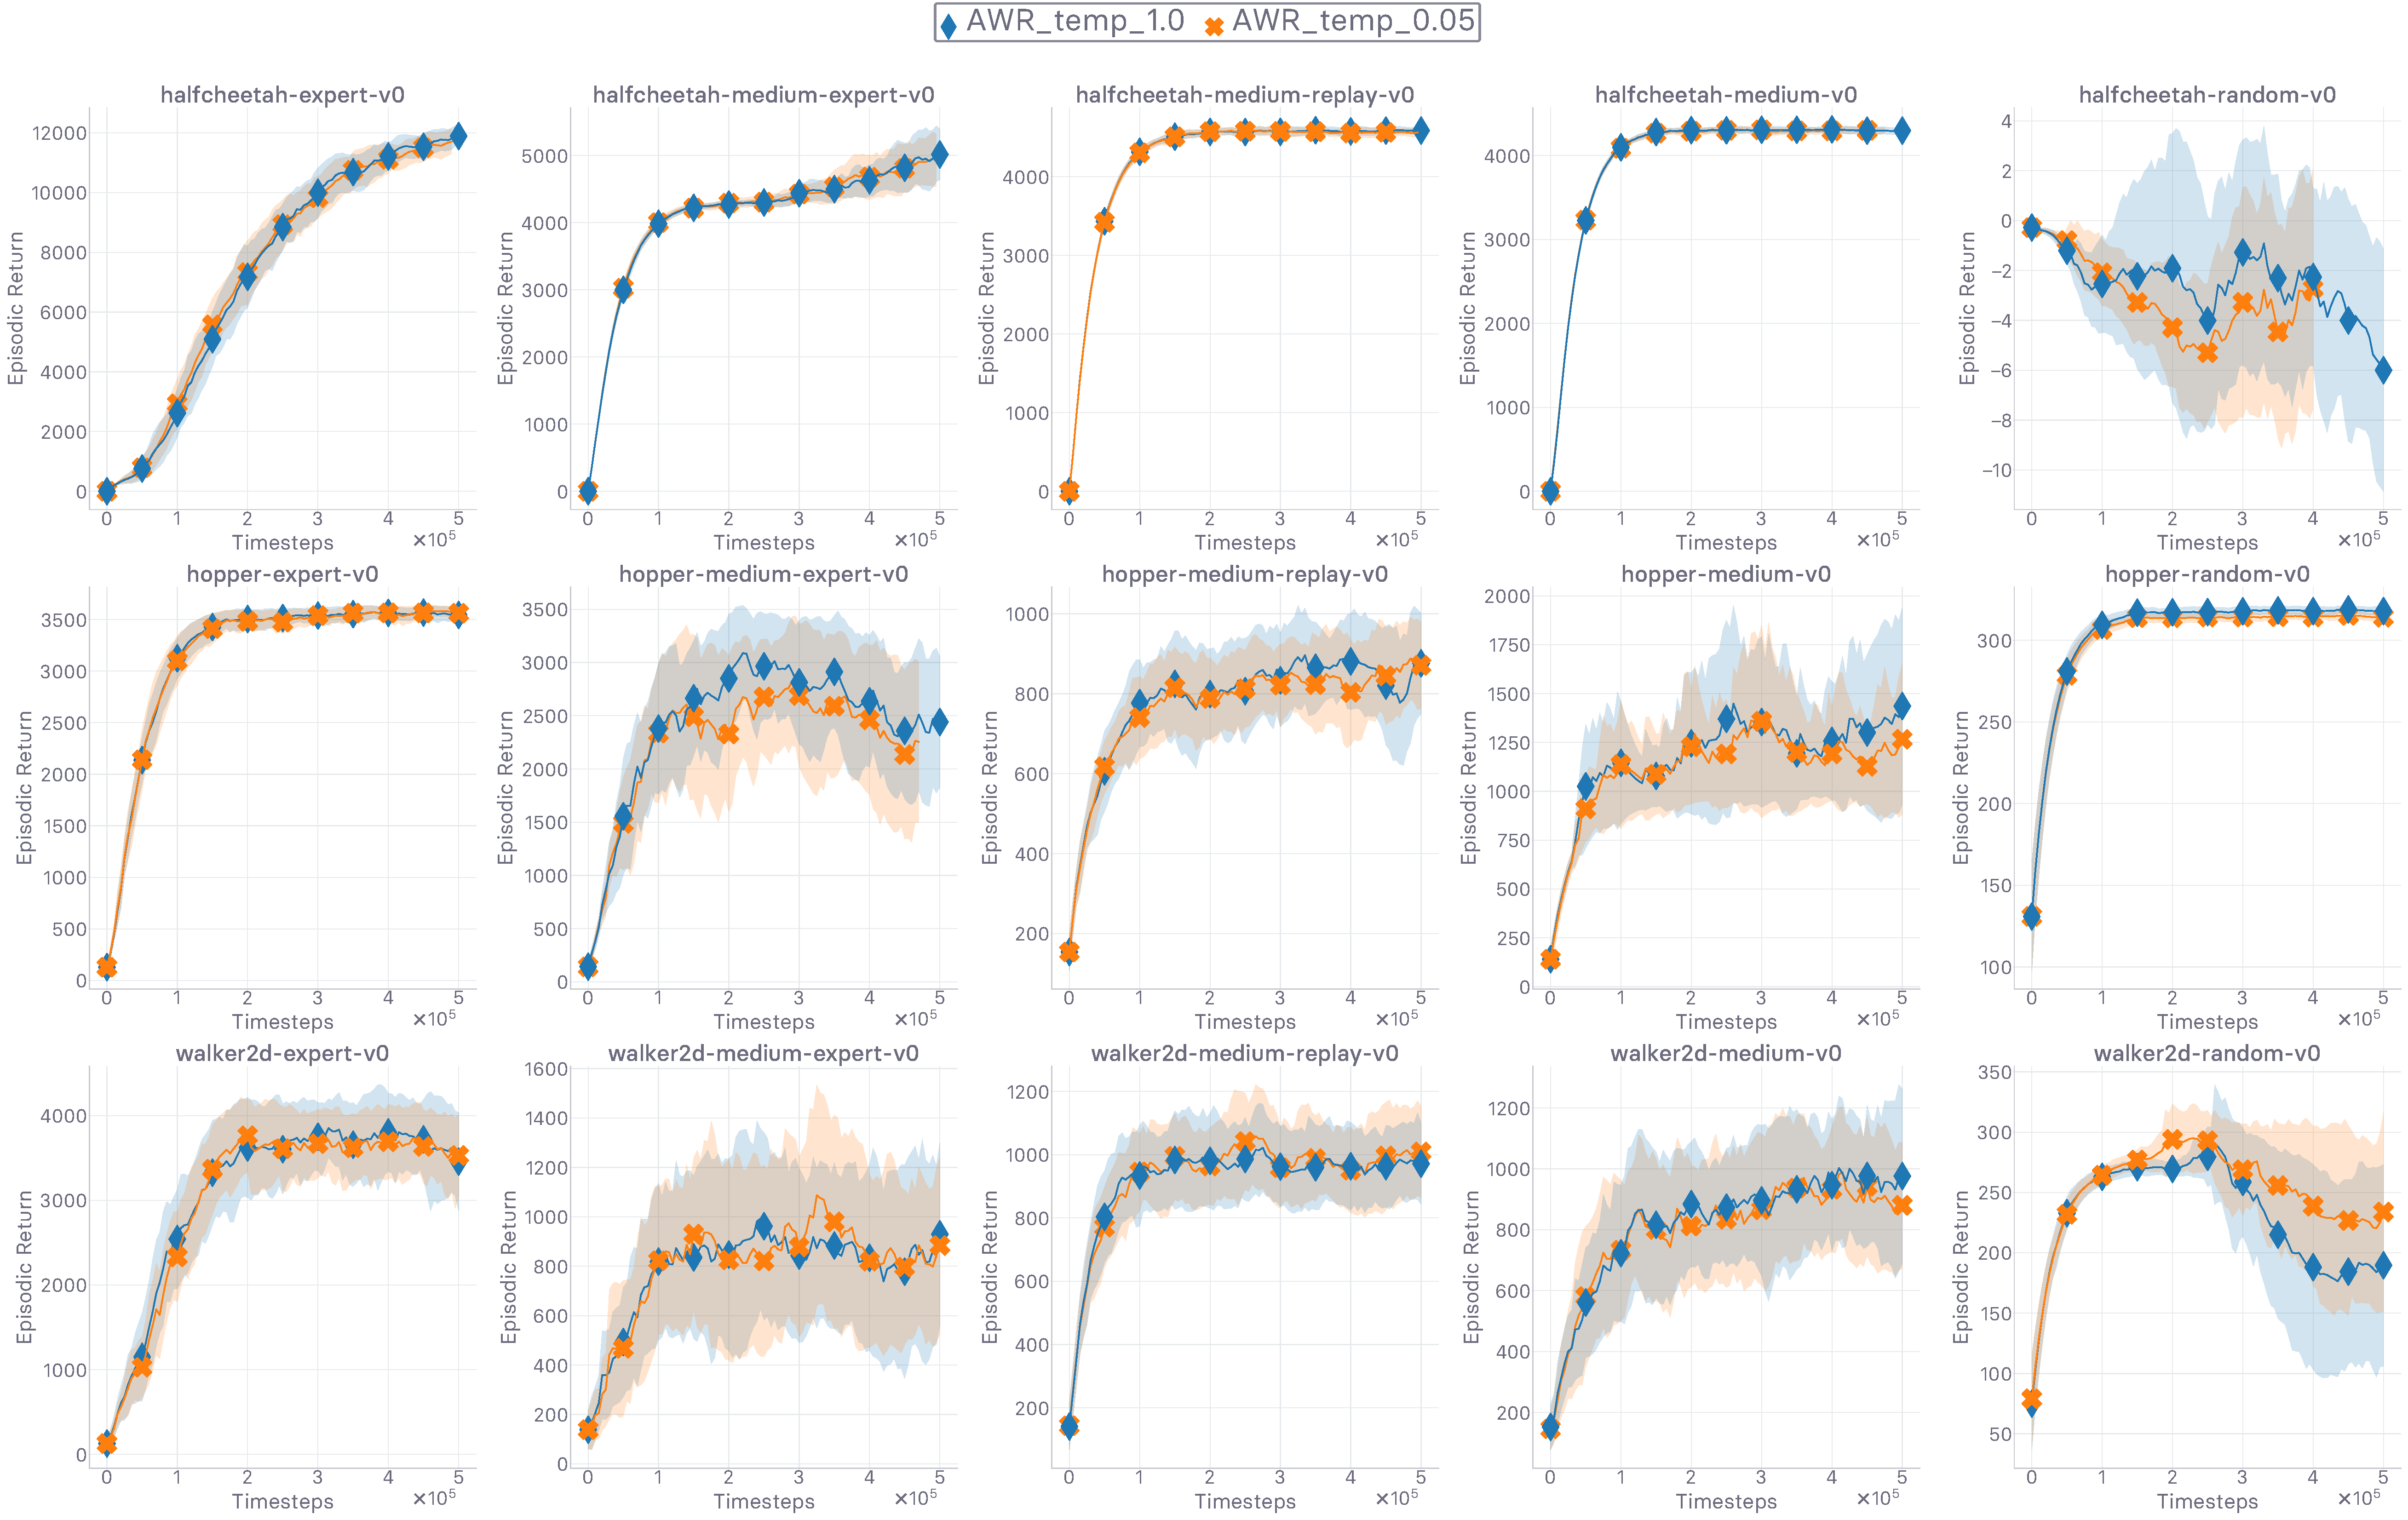
\includegraphics{Plots/awr_sweep/plots_main_eval_env_ret_plot.pdf}}
  \caption{Sweep over the temperature $\tau$ used in the advantage-based exponential weights objective of AWR.
  Note some sets of runs (\textit{e.g.} top-right sub-plot) terminated early due to an issue on
  our computational infrastructure.
  Since the results were conveying the message we wanted to communicate (the temperature has little to no
  impact on performance), we did not deem it necessary to re-run these experiments.
  Runtime is 12 hours. Best seen in color.}
  \label{awrsweep:barplot}
\end{figure}
